\section{Contraposée du théorème de Thalès}
    \subsection{Énoncé}
        \begin{theoreme}[\admis]
            Si dans un triangle $ABC$ :
            \begin{itemize}
                \item $M$ est un point du côté $[AB]$ distinct de $A$ et $B$.
                \item $N$ est un point du côté $[AC]$ distinct de $A$ et $C$.
                \item $\dfrac{AM}{AB} \neq \dfrac{AN}{AC}$.       
            \end{itemize}
            \medskip
            alors les droites $(BC)$ et $(MN)$ ne sont pas parallèles.
        \end{theoreme}

    \subsection{Exemple de rédaction}

        \begin{methode*1}[Justifier que deux droites ne sont pas parallèles]
            \begin{multicols}2
                \begin{itemize}
                    \item Identifier les deux triangles.                                    
                    \item Calculer les rapports de longueurs non portées par les droites candidates.
                    \item Invoquer la contraposée du théorème de Thalès ou le théorème lui-même.
                \end{itemize}
            \end{multicols}

            \exercice

            \begin{minipage}{8cm}
                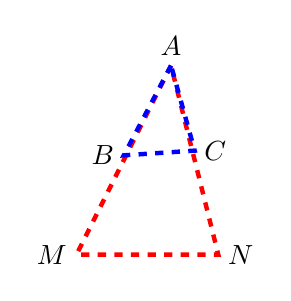
\begin{tikzpicture}[scale = 0.3]
                    % \draw[help lines, color=black!30, dashed] (0,0) grid (12,14);        
                    \coordinate[label=above:$A$] (A) at (7,13);
                    % \coordinate[label=left:$(d')$] (d') at (6.7,14);
                    % \coordinate[label=right:$(d)$] (d) at (7.5,14);
                    \coordinate[label=right:$N$] (N) at (9,5);
                    \coordinate[label=left:$M$] (M) at (3,5);
                    \coordinate[label=left:$B$] (B) at (5,9.2);
                    \coordinate (M1) at (4,5);
                    \coordinate[label=right:$C$] (C) at (8,9.4);
                    \coordinate (N1) at (10,5);
        
                    \tkzDrawSegment(A,M);
                    \tkzDrawSegment(A,N);
                    \tkzDrawSegment(M,N);
                    \tkzDrawSegment(B,C);
                    % \tkzDrawSegment(M1,N1);     
                    \draw[dashed, color=red, ultra thick] (A)--(M)--(N)--(A);
                    \draw[dashed, color=blue, ultra thick] (A)--(B)--(C)--(A);
                \end{tikzpicture}
            \end{minipage}
            \begin{minipage}{8cm}
                \begin{itemize}
                    \item $A$, $B$, $M$ sont alignés.
                    \item $A$, $C$, $N$ sont alignés.
                    \item $AB=\Lg{11.9}$ ; $AM=\Lg{35}$. 
                    \item $AC=\Lg{18.2}$ ; $AN=\Lg{52}$.
                \end{itemize}

                % \vspace*{1cm}
                Démontrer que les droites $(MN)$ et $(BC)$ 
                
                ne sont pas parallèles.
            \end{minipage}
            
            \correction
            Dans le configuration ci-dessus : 
            \begin{itemize}
                \item les deux triangles sont \textcolor{red}{$AMN$} et \textcolor{blue}{$ABC$}.
                \item $B \in [AM]$ et $C \in [AN]$.
                \item D'une part $\dfrac{\textcolor{blue}{AB}}{\textcolor{red}{AM}} = \dfrac{\textcolor{blue}{11,9}}{\textcolor{red}{35}}=0,34$
                \hfill
                D'autre part $\dfrac{\textcolor{blue}{AC}}{\textcolor{red}{AN}} = \dfrac{\textcolor{blue}{18,2}}{\textcolor{red}{52}}=0,35$
            \end{itemize}

            \begin{remarque}
                Les deux rédactions suivantes sont valables.
            \end{remarque}
            
            \hspace*{0.5cm}

            \begin{minipage}{8cm}
                \textbf{or}, si le droites $(MN)$ et $(BC)$ étaient parallèles, d'après le théorème de Thalès, il y aurait égalité des deux rapports
                précédents. Comme ce n'est pas le cas, c'est que \psshadowbox{les droites $(MN)$ et $(BC)$ ne sont pas parallèles}.
    
            \end{minipage}
            \hspace*{0.5cm}
            \vrule
            \hspace*{0.5cm}
            \begin{minipage}{8cm}
                Les rapports précédents étant différents, d'après la contraposée du théorème de Thalès, on peut conclure que \psshadowbox{les droites $(MN)$ et $(BC)$ ne sont pas parallèles}.
            \end{minipage}
        \end{methode*1}

        % \begin{remarque}
        %     D'une façon générale, la contraposée d'un théorème permet d'affirmer que les conditions
        %     de ce théorème sont fausses dès que l'unes des conclusions de ce théorème n'est pas vérifiée.
        % \end{remarque}


% \subsection{Sous-section 1.1}
% \begin{definition}[Titre optionnel]
%     Dans le cours, on utilise assez souvent des cadres du type
%     définition (comme ici par exemple).    
% \end{definition}
% \begin{remarque}
%     Ceci est une remarque utilisant une commande du paquet profcollege.
    
%     \begin{center}
%       Truc centré
%     \end{center}


% \end{remarque}
% \begin{propriete}[Titre optionnel]
%   Dans le cours, on utilise assez souvent des cadres du type
%   définition, comme ici par exemple pour une propriete.
% \end{propriete}
% \begin{remarques}
%   \begin{itemize}
%     \item remarque.
%     \item remarque.
%   \end{itemize}
% \end{remarques}

% \subsection{Sous-section 1.2}
% \begin{theoreme}[Titre optionnel]
%   Dans le cours, on utilise assez souvent des cadres du type
%   définition, comme ici par exemple pour un théorème.
% \end{theoreme}
% \begin{notation}
%   notation
% \end{notation}
% \begin{notations}
%   \begin{itemize}
%     \item notation.
%     \item notation.
%   \end{itemize}
% \end{notations}
% \begin{preuve}
%   Ceci est une preuve\par Deuxième ligne de la preuve
% \end{preuve}
% \begin{exemple}
%   Texte de l’exemple
%   \correction
  
% \end{exemple}

% \begin{exemple*1}
%   \phantom{rrr}
%   Texte

%   \correction
%   \phantom{rrr}
%   Texte  
  
% \end{exemple*1}

% \begin{exemple}[0.6]
%   Texte de l’exemple très long sur une ligne, très très très long.
%   On peut modifier la répartition horizontale  à l'aide d'un argument optionnel valant par défaut 0,4, valant ici 0,6.
%   \correction
%   Texte de la correction en vis à vis
% \end{exemple}
% \section{Section 2}
% \subsection{Sous-section 2.1}
% Quatre affichages prévus pour les méthodes.

% \begin{methode}[Titre de la méthode]
%     \Papiers[Largeur=10,Hauteur=5,Couleur=Olive]
    
%     Texte introductif
%     \exercice
%     Texte de l’exercice
%     \correction
%     Texte de la correction sur un minimum de trois lignes pour faire la
%     différence entre vis-à-vis et double colonne. C’est l’endroit de la
%     coupure qui va différer.
% \end{methode}

% \begin{methode*1}[Titre de la méthode*1]
%     Texte introductif
%     \exercice
%     Texte de l’exercice
%     \correction
%     Texte de la correction sur un minimum de trois lignes pour faire la
%     différence entre vis-à-vis et double colonne. C’est l’endroit de la
%     coupure qui va différer.
% \end{methode*1}

% \subsection{Sous-section 2.2}
% \begin{methode*2}[Titre de la méthode*2]
%     Texte introductif
%     \exercice
%     Texte de l’exercice
%     \correction
%     Texte de la correction sur un minimum de trois lignes pour faire la
%     différence entre vis-à-vis et double colonne. C’est l’endroit de la
%     coupure qui va différer.
% \end{methode*2}

% \begin{methode*2*2}[Dernière méthode  \MethodeRefExercice{exoN1-exemple1} \MethodeRefExercice{exoN1-exemple2}]
%     \exercice
%     \label{methodeN1-exemple}
%     Texte du premier exercice
%     \correction
%     Correction du premier exercice
%     \exercice
%     Texte du deuxième exercice
%     \correction
%     Texte de la correction du deuxième exercice sur un minimum de trois
%     lignes pour faire la différence entre vis-à-vis et double
%     colonne. C’est l’endroit de la coupure qui va différer.
% \end{methode*2*2}